\chapter{The AILS-NTUA System Architecture}
\label{chapter:system}

This chapter provides an exhaustive technical description of the AILS-NTUA architecture developed for multi-turn conversational Retrieval-Augmented Generation. We proceed from architectural principles (Section~\ref{sec:arch-overview}) to the multi-strategy retrieval engine addressing Task~A (Section~\ref{sec:retrieval-pipeline}), the multi-stage agentic generation pipeline addressing Task~B (Section~\ref{sec:generation-pipeline}), and finally the unified end-to-end system with its multi-layer answerability gate addressing Task~C (Section~\ref{sec:e2e-system}). Throughout, we use the notation established in Chapter~4: $H_t$ for dialogue history, $q_t$ for the active query, $\mathcal{D}_t$ for retrieved passages, and $y_t$ for the generated response at turn $t$.

%==============================================================
\section{Architectural Overview and System Principles}
\label{sec:arch-overview}
%==============================================================

The design of AILS-NTUA addresses the two systematic vulnerabilities of multi-turn dialogue identified in Chapter~4---unresolved cross-turn dependency and the resulting context drift in retrieval, and the answer-or-abstain decision of end-to-end RAG---by replacing brittle, monolithic components with an engineered chain of decentralized, task-specific modules. Rather than treating retrieval and generation as opaque black boxes to be scaled with larger models, the architecture is governed by two orthogonal design principles that recur throughout this chapter.

\paragraph{Principle 1 --- Query Diversity over Retriever Diversity.}
A common architectural instinct when facing retrieval brittleness is to ensemble multiple heterogeneous retrievers (e.g., a sparse lexical model, a dense neural model, and a learned sparse model), on the assumption that diverse retrieval signals are strictly complementary. Under the benchmark's official relevance judgments, our ablations (Section~\ref{sec:taskA-ablations}) do not support this assumption in the multi-turn setting: heterogeneous retriever ensembling raises deep recall but lowers top-rank precision, displacing high-confidence hits from the top of the ranking (subject to the pooling-bias caveat of Section~\ref{sec:pooling-bias}). AILS-NTUA instead fixes the search index onto a single corpus-aligned encoder, the strongest in our retriever comparison (ELSER~v1, Section~\ref{sec:taskA-ablations}), and diversifies the \emph{query side} instead, projecting the same underspecified utterance across five complementary LLM-generated reasoning paths (Section~\ref{sec:retrieval-pipeline}).

\paragraph{Principle 2 --- Deferred Answer Commitment via Multi-Agent Verification.}
Rather than committing to a single generation pass, the system insulates factual synthesis from full-document noise through a sequence of evidence bottlenecks: sentence-level span extraction, parallel drafting of multiple candidate responses, and programmatic validation by a persona-conditioned judge ensemble before any answer is finalized. This mirrors the LLM-as-a-Judge paradigm reviewed in Section~3.4.2, extended here with an explicit extractiveness-calibration objective (Section~\ref{sec:generation-pipeline}).

These two principles map directly onto the three functional modules of the system, which correspond one-to-one with the MTRAGEval subtask specification of Section~4.1: the \textbf{Multi-Strategy Retrieval Pipeline} (Task~A, Figure~\ref{fig:taskA-en}), the \textbf{Multi-Stage Agentic Generation Pipeline} (Task~B, Figure~\ref{fig:taskB-en}), and the \textbf{Unified End-to-End System} (Task~C, Figure~\ref{fig:taskC-en}), which composes the first two modules and adds a dedicated answerability-gating layer. Figure~\ref{fig:overview-en} summarizes how these three modules relate before the following sections detail each one individually.

\begin{figure}[h]
\centering
\begin{tikzpicture}[
  node distance=6mm,
  box/.style={draw, rounded corners, align=center, minimum height=8mm, font=\footnotesize, fill=blue!6},
  sub/.style={draw, rounded corners, align=center, minimum height=8mm, font=\scriptsize},
  arr/.style={-Stealth, thick}
]
\node[box] (in) {Query $q_t$ + History $H_t$};
\node[sub, below=of in, fill=blue!8, text width=58mm] (a) {\textbf{Task A} --- Multi-Strategy Retrieval Pipeline (Sec.~5.2, Fig.~\ref{fig:taskA-en})};
\node[sub, below=of a, fill=orange!8, text width=58mm] (draft) {\textbf{Task B}, Stages 2--3: span extraction and dual-candidate drafting (Sec.~5.3, Fig.~\ref{fig:taskB-en})};
\node[sub, below=of draft, fill=red!8, text width=58mm] (gate) {Multi-Layer Answerability Gate (Sec.~5.4)};
\node[sub, below left=6mm and -10mm of gate, fill=orange!8, text width=30mm] (refusal) {Unanswerable: calibrated refusal};
\node[sub, below right=6mm and -10mm of gate, fill=orange!8, text width=30mm] (b) {Answerable: \textbf{Task B}, Stages 4--5 (selection, micro-adjustment)};
\node[box, below=16mm of gate, fill=green!10] (out) {Response $y_t$ / Refusal};
\draw[arr] (in) -- (a);
\draw[arr] (a) -- (draft);
\draw[arr] (draft) -- (gate);
\draw[arr] (gate) -- node[left, font=\scriptsize] {no} (refusal);
\draw[arr] (gate) -- node[right, font=\scriptsize] {yes} (b);
\draw[arr] (refusal.south) |- (out.west);
\draw[arr] (b.south) |- (out.east);
\end{tikzpicture}
\caption{High-level composition of the three functional modules of AILS-NTUA. Task~A (retrieval) and Task~B (reference-grounded generation) are each evaluated independently in their standalone configurations; Task~C composes both: span extraction and dual-candidate drafting run first, because the answer-level judge of the Multi-Layer Answerability Gate (Sec.~\ref{sec:e2e-system}, Fig.~\ref{fig:taskC-en}) inspects a drafted answer; the gate then either lets the turn finish the remaining Task~B stages or replaces the draft with a calibrated refusal.}
\label{fig:overview-en}
\end{figure}

%==============================================================
\section{The Multi-Strategy Retrieval Pipeline (Task A)}
\label{sec:retrieval-pipeline}
%==============================================================

The retrieval pipeline transforms a brief, context-dependent query $q_t$ and its conversation history $H_t$ into a stable, noise-resilient ranked list of passages $\mathcal{D}_t$, through a four-stage process: query rewriting, first-stage sparse retrieval, cross-encoder reranking, and hierarchical rank fusion.

\subsection{The Five-Pronged Query Rewriting Engine}
\label{subsec:rewriting-engine}

At turn $t$, the historical window $H_t$ (truncated to the six most recent user turns and up to three assistant turns, per the ablation of Table~\ref{tab:history-ablation}) and the active utterance $u_t$ are passed to a query rewriting module instantiated on DeepSeek-V3.2 at temperature $T{=}0.0$. The module executes five independent prompt tracks \emph{simultaneously}, each engineered to target a distinct failure mode identified in Section~\ref{sec:nonstandalone-phenomena}:

\begin{description}
    \item[Minimal Reformulation ($q_t^{\min}$).] Resolves purely anaphoric tokens and structural ellipsis, converting the query into a grammatically complete, standalone question while preserving the user's original phrasing as closely as possible. This strategy is deliberately conservative---its system prompt explicitly instructs the model \emph{not} to introduce new terminology---so as to avoid the over-expansion failure mode observed with weaker rewriting models (Section~6.2).
    \item[Corpus-Specific Reformulation ($q_t^{\text{corp}}$).] Maps the user's conversational terminology onto the formal register, synonym sets, and structural metadata conventions of the active domain corpus (e.g., translating informal forum phrasing in FiQA into standard financial terminology). Domain-specific preservation rules govern what must be kept verbatim---entity variants and temporal phrasing for ClapNQ, exact amounts and tickers for FiQA, program names and form identifiers for Govt, and error codes and CLI flags for Cloud.
    \item[Hypothetical Document Embedding ($q_t^{\text{hyde}}$).] Following the HyDE paradigm introduced in Section~3.1.4, instructs the LLM to generate a brief, zero-shot hypothetical answer passage based entirely on its parametric knowledge. This hypothetical block acts as a semantic proxy that pivots the matching problem from question-to-passage to answer-to-passage similarity.
    \item[Chain-of-Thought Decomposition ($q_t^{\text{cot}}$).] Triggers a sequential reasoning prompt that first identifies the explicit sub-questions and intermediate information primitives necessary to answer $q_t$, before producing the final rewritten query. This captures the underlying informational structure of complex or comparative questions that a single surface-level rewrite would miss.
    \item[Anchor Keyword Targeting ($q_t^{\text{key}}$).] Extracts static, high-discrimination alphanumeric sequences---entity names, acronyms, error codes, system identifiers---that function as structural indexing anchors, particularly valuable for the technical, code-dense Cloud domain where semantic paraphrase strategies are least reliable.
\end{description}

Each of the five strategies produces both a rewritten query string and a binary standalone/non-standalone classification, returned as structured JSON to guarantee downstream parseability. All five prompt templates share a common XML-structured scaffold (system instructions, few-shot demonstration, structured output schema) but differ in their preservation rules and the amount of assistant-turn context supplied, summarized in Table~\ref{tab:rewrite-config-en}.

\begin{table}[h]
\centering
\small
\begin{tabular}{lcl}
\toprule
\textbf{Strategy} & \textbf{Assistant Turns} & \textbf{Key Behavior} \\
\midrule
Minimal & 3 & Coreference and ellipsis resolution only \\
Corpus-Specific & 0--3 & Domain-aware terminology mapping \\
Chain-of-Thought & 3 & Explicit intermediate reasoning trace \\
HyDE & 3 & Zero-shot hypothetical answer passage \\
Anchor-Keyword & 1 & Entity and intent term extraction \\
\bottomrule
\end{tabular}
\caption{Configuration of the five query rewriting strategies. The amount of assistant-turn context supplied is tuned per strategy: Anchor-Keyword requires minimal context since it operates primarily on the current utterance, while reasoning-heavy strategies (Minimal, CoT, HyDE) benefit from a wider historical window.}
\label{tab:rewrite-config-en}
\end{table}

\subsection{Validating the Necessity of LLM-Based Rewriting}
\label{subsec:rewriting-necessity}

Before committing to the five-strategy design of Table~\ref{tab:rewrite-config-en}, we first verified
that instruction-following LLM rewriting is actually \emph{necessary}, rather than assuming it a
priori. Table~\ref{tab:rewrite-necessity-en} compares the unaugmented baseline against a non-LLM
neural rewriter (FlanT5, fine-tuned for query reformulation) and an annotator-replica prompt that
reproduces the query rewriting instructions used during MTRAG's own data collection process
\citep{katsis2025mtrag}.

\begin{table}[h]
\centering
\small
\begin{tabular}{lcc}
\toprule
\textbf{Method} & \textbf{Recall@5} & \textbf{nDCG@5} \\
\midrule
Unaugmented baseline & 0.483 & 0.444 \\
FlanT5 (non-LLM neural rewriter) & 0.462 & 0.421 \\
Annotator-replica prompt & 0.513 & 0.470 \\
Minimal (ours, DeepSeek-V3.2) & 0.527 & 0.487 \\
Corpus-Specific (ours, best single strategy) & 0.541 & 0.498 \\
\bottomrule
\end{tabular}
\caption{Rewriting method necessity check, development set. FlanT5 falls \emph{below} the unaugmented
baseline, confirming that poorly calibrated rewriting actively harms retrieval; every LLM-based
strategy improves over both the baseline and the annotator-replica prompt.}
\label{tab:rewrite-necessity-en}
\end{table}

The result is a genuine negative finding for the smaller, non-LLM rewriter: FlanT5 degrades
Recall@5 \emph{below} the unaugmented baseline ($0.483 \rightarrow 0.462$), confirming that
rewriting is not unconditionally beneficial---a reformulation model without strong instruction-following
capability introduces more query drift than it resolves, over-generalizing the original intent rather
than sharpening it. This ruled out non-LLM rewriters and classical pseudo-relevance feedback early in
development (see also the negative PIR result of Section~\ref{sec:pir}, which encounters a structurally
related failure mode) and confined the design space explored in Section~\ref{subsec:rewriting-engine}
to prompt-level variation over a single strong instruction-following backbone.

Table~\ref{tab:rewrite-example-en} illustrates the qualitative behavior of each strategy on a
representative non-standalone Cloud-domain query, where \textit{the pricing} refers to an entity
(IBM Cloud Object Storage) introduced several turns earlier in the conversation.

\begin{table}[h]
\centering
\small
\begin{tabular}{p{2.6cm}p{9.6cm}}
\toprule
\textbf{Strategy} & \textbf{Example Output} \\
\midrule
Original & ``What about the pricing?'' \\
Minimal & ``What is the pricing for IBM Cloud Object Storage?'' \\
Corpus-Specific & ``IBM Cloud Object Storage pricing tiers and cost structure'' \\
HyDE & ``IBM Cloud Object Storage offers flexible pricing based on storage class, including Standard, Vault, and Cold Vault tiers\ldots'' \\
Chain-of-Thought & ``Need: storage costs, transfer fees, API pricing $\rightarrow$ IBM Cloud Object Storage full pricing breakdown'' \\
Anchor-Keyword & ``IBM Cloud Object Storage pricing cost GB month tier'' \\
\bottomrule
\end{tabular}
\caption{Representative reformulations of a non-standalone Cloud-domain query. Each strategy resolves
the underspecified reference to \textit{the pricing} differently, illustrating the complementary
failure-mode coverage that motivates fusing all five under Nested RRF (Section~\ref{subsec:nested-rrf})
rather than selecting a single ``best'' strategy.}
\label{tab:rewrite-example-en}
\end{table}

\subsection{First-Stage Learned Sparse Search and Cross-Encoder Reranking}
\label{subsec:reranking}

Each of the five generated queries $q_t^m$ (for $m \in \{\min, \text{corp}, \text{hyde}, \text{cot}, \text{key}\}$) is issued \emph{independently} to the ELSER~v1 learned sparse retriever, which scans the corpus-specific index and surfaces the top-$N$ ($N{=}100$) document passages according to its learned term-expansion weights (Section~3.1.3).

To sharpen top-tier precision beyond what the sparse retriever alone provides, the top-$60$ passages from each individual track are routed to a specialized cross-encoder reranker~\citep{nogueira2019passage, nogueira2020monot5}, instantiated as \textbf{Cohere Rerank~v4}. The cross-encoder computes full cross-attention over the concatenated query--passage token sequence, returning a finely calibrated relevance score that the sparse retriever's bag-of-weights scoring cannot capture---in particular, negation, multi-hop entity disambiguation, and fine-grained numerical comparison.

The reranker's output is \emph{not} used as a standalone ranking signal. As shown in Section~\ref{sec:taskA-ablations} (Table~\ref{tab:reranking-alone-en}), replacing the retriever entirely with a cross-encoder lowers Recall@5 by $4.6$--$10.6$ points ($8.7$--$20.0\%$ relative) compared with the sparse retriever baseline, despite the cross-encoder's strong performance on standard, static IR benchmarks. Instead, retriever and reranker signals are fused through a weighted RRF combination:
\begin{equation}
\text{Score}(d) = \frac{1}{k + r_{E}(d)} + \alpha \cdot \frac{1}{k + r_{R}(d)}
\label{eq:hybrid-rerank}
\end{equation}
where $r_E(d)$ and $r_R(d)$ denote the ranks assigned to document $d$ by the ELSER retriever and the Cohere reranker respectively, $k$ controls rank-decay steepness ($k{=}60$), and $\alpha$ balances the relative contribution of the two signals ($\alpha{=}0.5$, tuned on the development set). We interpret this asymmetry---strong \emph{fused} contribution but weak \emph{standalone} contribution---as evidence that the cross-encoder functions as a complementary refinement filter operating on an already-relevant candidate pool, rather than as an independent source of retrieval recall; a distinction with direct implications for practitioners tempted to deploy reranker-only pipelines in low-resource settings.

\subsection{The Nested Reciprocal Rank Fusion (Nested RRF) Algorithm}
\label{subsec:nested-rrf}

Rather than combining the five reranked candidate lists under a single, flat RRF aggregation (Section~3.2.1), the pipeline introduces a hierarchical, two-level \textbf{Nested RRF} structure, designed to limit the influence of the exploratory reformulations. The design rests on the expectation, motivated in Section~3.2.2, that Minimal and Corpus-Specific reformulations behave consistently across turns, whereas HyDE, Chain-of-Thought, and Anchor-Keyword are more volatile---helpful on some turns and misleading on others, depending on whether the generated hypothesis or reasoning trace matches the true topic. We did not measure per-turn variance directly; the per-strategy results of Section~\ref{sec:taskA-ablations} show that HyDE is the weakest single strategy in every domain, while the complete fusion still exceeds the best single strategy.

Algorithm~\ref{alg:nested-rrf} formalizes the two-level fusion procedure. At \textbf{Level~1}, the three exploratory tracks are pre-aggregated via flat RRF into a single intermediate ``weak consensus'' ranking, using an internal smoothing constant $k_{\text{internal}}{=}40$; this pre-aggregation step is intended to absorb the idiosyncratic noise of any single exploratory strategy before it can independently displace a high-confidence document from the final top-$k$. At \textbf{Level~2}, this consensus ranking is fused with the two conservative strategies under domain-specific weights $w_s^{(c)}$, producing the final passage ranking $\mathcal{D}_t$.

\begin{algorithm}[h]
\caption{Nested Reciprocal Rank Fusion}
\label{alg:nested-rrf}
\KwIn{Reranked lists $\mathcal{L}_{\min}, \mathcal{L}_{\text{corp}}, \mathcal{L}_{\text{key}}, \mathcal{L}_{\text{hyde}}, \mathcal{L}_{\text{cot}}$; constant $k$; corpus-specific weights $w_s^{(c)}$}
\KwOut{Unified ranked passage list $\mathcal{D}_t$}
\Comment{Level 1: pre-aggregate high-variance exploratory paths}
\For{each document $d \in \mathcal{L}_{\text{hyde}} \cup \mathcal{L}_{\text{cot}} \cup \mathcal{L}_{\text{key}}$}{
    $\text{Score}_{\text{L1}}(d) \gets \dfrac{1}{k_{\text{internal}} + \text{rank}_{\text{hyde}}(d)} + \dfrac{1}{k_{\text{internal}} + \text{rank}_{\text{cot}}(d)} + \dfrac{1}{k_{\text{internal}} + \text{rank}_{\text{key}}(d)}$\;
}
$\mathcal{L}_{\text{consensus}} \gets \text{SortDocumentsByScore}(\text{Score}_{\text{L1}})$\;
\Comment{Level 2: final aggregation with low-variance stable paths}
\For{each document $d \in \mathcal{L}_{\min} \cup \mathcal{L}_{\text{corp}} \cup \mathcal{L}_{\text{consensus}}$}{
    $\text{Score}_{\text{final}}(d) \gets \displaystyle\sum_{s \in \{\min,\, \text{corp},\, \text{consensus}\}} \dfrac{w_s^{(c)}}{k_{\text{final}}^{(c)} + \text{rank}_s(d)}$\;
}
$\mathcal{D}_t \gets \text{SortDocumentsByScore}(\text{Score}_{\text{final}})[\text{top-}k]$\;
\Return{$\mathcal{D}_t$}
\end{algorithm}

The domain-specific weights $w_s^{(c)}$ and final-stage smoothing constants $k_{\text{final}}^{(c)}$, reported in Table~\ref{tab:nested-rrf-weights-en}, were tuned by grid search exclusively on the development set. The pattern of tuned values is itself interpretable: formal, terminology-dense domains (Govt, Cloud) assign the largest weight to the conservative Minimal strategy, which preserves exact domain terminology, whereas FiQA---the domain with the largest vocabulary gap between informal user language and formal document content---assigns comparatively more weight to the exploratory weak-consensus group, where semantic paraphrase diversity is most valuable. We note, however, that this tuning is a refinement rather than a prerequisite: in development runs, uniform weights across all four domains lowered Recall@5 by less than $1\%$ relative to the tuned configuration (this comparison is not tabulated). The precise weight values therefore matter little; whether the hierarchical structure itself improves over a flat fusion of the same five lists was not isolated (Section~\ref{sec:taskA-ablations}).

\begin{table}[h]
\centering
\small
\begin{tabular}{lcccc}
\toprule
\textbf{Parameter} & \textbf{ClapNQ} & \textbf{FiQA} & \textbf{Govt} & \textbf{Cloud} \\
\midrule
$k_{\text{final}}^{(c)}$ & 20 & 60 & 40 & 20 \\
$w_{\text{Minimal}}$ & 0.55 & 0.45 & 0.65 & 0.65 \\
$w_{\text{Corpus-Spec}}$ & 0.40 & 0.40 & 0.25 & 0.30 \\
$w_{\text{WeakConsensus}}$ & 0.05 & 0.15 & 0.10 & 0.05 \\
\bottomrule
\end{tabular}
\caption{Nested RRF parameters tuned per corpus on the development set. Formal, terminology-stable domains (Govt, Cloud) weight the conservative Minimal strategy most heavily; FiQA, with the widest vocabulary gap, allocates the largest share to the exploratory weak-consensus group.}
\label{tab:nested-rrf-weights-en}
\end{table}

\begin{figure}[h]
\centering
\begin{tikzpicture}[
  node distance=6mm and 8mm,
  box/.style={draw, rounded corners, align=center, minimum height=8mm, font=\footnotesize, fill=blue!6},
  strat/.style={draw, rounded corners, align=center, minimum height=7mm, font=\scriptsize, fill=orange!8},
  arr/.style={-Stealth, thick}
]
\node[box] (in) {Query $q_t$ + History $H_t$};
\node[box, below=of in] (rw) {1. Multi-Strategy Rewriting};
\node[strat, below left=4mm and -8mm of rw] (s1) {Minimal};
\node[strat, right=2mm of s1] (s2) {Corpus-Sp.};
\node[strat, right=2mm of s2] (s3) {HyDE};
\node[strat, right=2mm of s3] (s4) {CoT};
\node[strat, right=2mm of s4] (s5) {Anchor-KW};
\node[box, below=14mm of rw] (ret) {2. Sparse Retrieval (ELSER v1) — top-100 per query};
\node[box, below=of ret] (rer) {3. Hybrid Reranking: Cohere Rerank v4 + w-RRF};
\node[box, below=of rer] (nrrf) {4. Nested RRF Fusion — per-corpus weights};
\node[box, below=of nrrf, fill=green!10] (out) {Top-$k$ Passages $\mathcal{D}_t$};
\draw[arr] (in) -- (rw);
\draw[arr] (rw) -- (s1); \draw[arr] (rw) -- (s2); \draw[arr] (rw) -- (s3);
\draw[arr] (rw) -- (s4); \draw[arr] (rw) -- (s5);
\draw[arr] ([yshift=-3mm]s1.south) -- (ret.north -| s1);
\draw[arr] ([yshift=-3mm]s3.south) -- (ret.north -| s3);
\draw[arr] (ret) -- (rer);
\draw[arr] (rer) -- (nrrf);
\draw[arr] (nrrf) -- (out);
\end{tikzpicture}
\caption{Task~A retrieval pipeline: five complementary reformulations are issued independently to ELSER~v1, followed by hybrid cross-encoder reranking and hierarchical Nested RRF fusion.}
\label{fig:taskA-en}
\end{figure}
\subsection{Conversation History Window Ablation}
\label{sec:history-ablation}

The query rewriting stage (Section~\ref{subsec:rewriting-engine}) requires access to prior conversation
turns to resolve coreferences and reconstruct standalone queries. We ablate the amount of history
provided to the rewriter along two independent axes: the number of user turns and the number of
assistant turns included in the prompt window. Table~\ref{tab:history-ablation} reports the results
under Minimal rewriting on the development set.

\begin{table}[h]
\centering
\begin{tabular}{lccc}
\toprule
\textbf{Configuration} & \textbf{User turns} & \textbf{Asst.\ turns} & \textbf{Recall@5} \\
\midrule
No history        & 0    & 0    & 0.490 \\
2 user turns       & 2    & 0    & 0.506 \\
4 user turns       & 4    & 0    & 0.528 \\
6 user turns       & 6    & 0    & 0.530 \\
8 user turns       & 8    & 0    & 0.528 \\
6u + 1 asst.\      & 6    & 1    & 0.528 \\
6u + 3 asst.\ (ours) & 6  & 3    & \textbf{0.533} \\
6u + 5 asst.\      & 6    & 5    & 0.532 \\
Full history       & all  & all  & 0.531 \\
\bottomrule
\end{tabular}
\caption{Conversation history window ablation (Minimal rewriting, development set). Recall@5
saturates after 4--6 user turns; assistant turns contribute negligible aggregate benefit beyond
one turn. This sweep was a separate run: under the same window, the Minimal strategy scores
$R@5{=}0.527$ in the strategy ablations (Table~\ref{tab:rewrite-ablation-en}), and the $0.006$ difference
could not be fully reconciled.}
\label{tab:history-ablation}
\end{table}

Two observations follow. First, retrieval quality is essentially insensitive to history beyond the
first 4--6 user turns: the gain from 4 to 6 user turns is only $+0.002$ R@5 (and $0.000$ from 4 to 8), an order of magnitude
smaller than the $+0.038$ gain from 0 to 4 turns. This saturation is consistent with the turn-depth
degradation pattern of Section~\ref{sec:turn-depth} — most coreferential ambiguity is resolved by
recent, not distant, context. Second, providing the \emph{full} unbounded history scores marginally
lower than the 6-turn window (0.531 vs.\ 0.533), a difference within run-to-run noise; a plausible reason is that early, no-longer-relevant
turns dilute the rewriter's effective attention over the truncated prompt budget. We adopt a window
of 6 user turns and 3 assistant turns as a conservative default: while assistant turns add negligible
\emph{aggregate} benefit, they remain necessary in edge cases where the user references an entity
introduced only in a prior assistant response, and their aggregate cost in prompt length is small.
%==============================================================
\section{The Multi-Stage Agentic Generation Pipeline (Task B)}
\label{sec:generation-pipeline}
%==============================================================

When the system is provided with a static, gold-standard reference block $\mathcal{D}_t^*$ (Task~B specification, Section~4.1.2), the generation module deliberately bypasses single-pass text generation, decomposing synthesis into five structured, sequential operational stages (Figure~\ref{fig:taskB-en}). This decomposition operationalizes Principle~2 of Section~\ref{sec:arch-overview}: no stage commits to the final answer until the preceding evidence-gathering and verification stages have executed.

\paragraph{Stage 1 --- Preliminary Answerability Classification.}
A lightweight verification prompt, executed on GPT-4o-mini, scans the reference passages $\mathcal{D}_t^*$. If the model determines with high confidence that the provided context lacks the information required to answer $q_t$, the pipeline halts immediately and returns a calibrated refusal string, avoiding the computational cost of the four downstream stages on a turn that cannot be answered regardless of generation quality.

\paragraph{Stage 2 --- Verbatim Evidence Span Extraction.}
To isolate the generator from document-level noise and mitigate the lost-in-the-middle effect~\citep{liu2024lost} discussed in Section~3.4.1, the context is routed through a fine-grained extraction bottleneck. The extraction model isolates the exact sentences or phrases within $\mathcal{D}_t^*$ that explicitly support an answer to $q_t$, returning a compressed, verbatim evidence set $\mathcal{S}_t = \{s_1, s_2, \dots, s_m\}$ with $m \leq 8$. As shown in Section~6.3, this single stage contributes the largest individual improvement of the entire generation pipeline ($+0.034$ Harmonic Mean), together with a $+0.041$ gain in the reference-less faithfulness metric $RL_F$---development-set support for the faithfulness part of Hypothesis~H2 of Section~4.4.

\paragraph{Stage 3 --- Dual-Candidate Drafting.}
The extracted spans $\mathcal{S}_t$ initialize two parallel generation tracks on GPT-4o, producing structurally distinct candidate responses:
\begin{itemize}
    \item \textbf{Deterministic Draft} ($y_t^{\text{det}}$, $T{=}0.0$): prioritizes literal precision, exact data formatting, and direct extraction from $\mathcal{S}_t$, maximizing reference-based overlap metrics at the cost of conversational fluency.
    \item \textbf{Stochastic Draft} ($y_t^{\text{sto}}$, $T{=}0.1$): targets conversational naturalness and discourse-level fluidity, at the cost of a marginally higher risk of drifting from the extracted evidence.
\end{itemize}
The narrow temperature gap between the two drafts ($0.0$ vs.\ $0.1$, rather than a wider spread) is itself a tuned design choice: wider gaps (e.g., $T_2{=}0.3$--$0.5$) were found in preliminary experiments (not retained) to degrade $RL_F$ without a compensating HM gain, since the stochastic draft's increased diversity comes disproportionately at the expense of grounding rather than genuine fluency variation.

\paragraph{Stage 4 --- Multi-Judge Selection Framework.}
The two candidates are evaluated by an ensemble of specialized judges, each processing the candidate text alongside the original query and the extracted evidence spans $\mathcal{S}_t$:
\begin{itemize}
    \item \textbf{Technical Judge} (DeepSeek-V3.2): evaluates absolute factual accuracy against $\mathcal{S}_t$ and flags internal contradictions or unsupported claims.
    \item \textbf{User Satisfaction Judge} (GPT-4o-mini, invoked stochastically on $60\%$ of turns): scores how completely and naturally the draft addresses the implicit information need, without evasive hedging language.
\end{itemize}
Selection additionally incorporates an \textbf{Extractiveness Shaping} term $\phi(r_4)$, which measures the $4$-gram token overlap $r_4$ between the candidate answer and the concatenated evidence spans, and penalizes deviation from an empirically calibrated ideal band:
\begin{equation}
\phi(r_4) =
\begin{cases}
-1.5 & \text{if } r_4 < 0.28 \quad \text{(under-extractive: hallucination risk)} \\
+2.5 & \text{if } 0.28 \leq r_4 \leq 0.38 \quad \text{(ideal)} \\
+1.5 & \text{if } 0.38 < r_4 \leq 0.50 \quad \text{(acceptable)} \\
+0.5 & \text{if } r_4 > 0.50 \quad \text{(over-extractive: robotic copying)}
\end{cases}
\label{eq:extractiveness-shaping}
\end{equation}
The ideal band $[0.28, 0.38]$ was calibrated directly against the empirical $4$-gram overlap of the development set's human reference answers, which average $36.2\%$. The function is deliberately \emph{asymmetric}: the penalty for under-extractive drafts ($-1.5$) is substantially larger in magnitude than the reduced reward for over-extractive ones ($+0.5$), reflecting our expectation that hallucination degrades downstream quality metrics more than mild verbatim repetition. Figure~\ref{fig:extractiveness-en} visualizes this shaping function. The prompts of Section~\ref{subsec:prompt-generation} refer to related but distinct values: the generation prompt asks for roughly $35\%$ verbatim overlap, i.e., close to the center of the ideal band, and the Technical Judge prompt states a wider tolerance of $28$--$45\%$; the band that actually enters the selection score is the one of Equation~\eqref{eq:extractiveness-shaping}.

\begin{figure}[h]
\centering
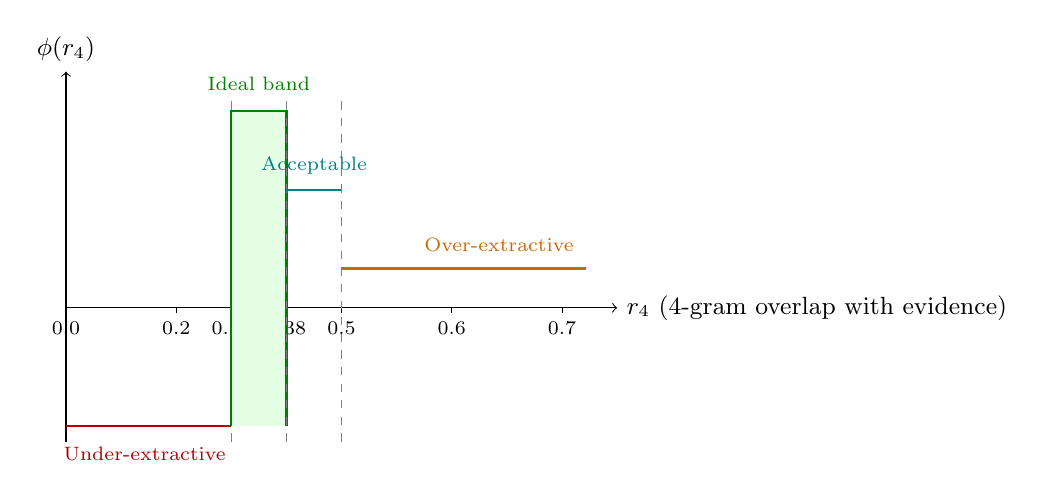
\begin{tikzpicture}
\draw[->] (0,0) -- (7,0) node[right, font=\small] {$r_4$ (4-gram overlap with evidence)};
\draw[->] (0,-1.7) -- (0,3) node[above, font=\small] {$\phi(r_4)$};
\foreach \x/\lbl in {0/0.0, 1.4/0.2, 2.1/0.28, 2.8/0.38, 3.5/0.5, 4.9/0.6, 6.3/0.7}
  \draw (\x,0) -- (\x,-0.06) node[below, font=\scriptsize] {\lbl};
\draw[thick, red!70!black] (0,-1.5) -- (2.1,-1.5);
\draw[dashed, gray] (2.1,-1.7) -- (2.1,2.7);
\draw[thick, green!50!black, fill=green!10] (2.1,-1.5) -- (2.1,2.5) -- (2.8,2.5) -- (2.8,-1.5);
\draw[thick, green!50!black] (2.1,2.5) -- (2.8,2.5);
\draw[dashed, gray] (2.8,-1.7) -- (2.8,2.7);
\draw[thick, teal] (2.8,1.5) -- (3.5,1.5);
\draw[dashed, gray] (3.5,-1.7) -- (3.5,2.7);
\draw[thick, orange!80!black] (3.5,0.5) -- (6.6,0.5);
\node[font=\scriptsize, red!70!black] at (1.0,-1.85) {Under-extractive};
\node[font=\scriptsize, green!50!black] at (2.45,2.85) {Ideal band};
\node[font=\scriptsize, teal] at (3.15,1.8) {Acceptable};
\node[font=\scriptsize, orange!80!black] at (5.5,0.8) {Over-extractive};
\end{tikzpicture}
\caption{The extractiveness shaping function $\phi(r_4)$: an asymmetric penalty/reward profile over the fraction of $4$-grams shared between a candidate answer and its extracted evidence spans, calibrated so that the ideal band $[0.28, 0.38]$ matches the empirical overlap of human reference answers ($36.2\%$).}
\label{fig:extractiveness-en}
\end{figure}

The composite selection score combines all three signals---technical judge score, signed user-preference indicator, and extractiveness shaping---together with an explicit penalty for residual hedging or refusal language detected via a forbidden-phrase filter (e.g., ``I am not sure'', ``it is unclear''), which we found to fire disproportionately on partially-answerable turns where the generator hedges despite the presence of usable evidence.

\paragraph{Stage 5 --- Micro-Adjustment and Post-Processing.}
The selected candidate undergoes a final, lightweight editing pass (GPT-4o-mini, $T{=}0.1$) that is applied \emph{only} when the answer violates one of three explicit length or extractiveness constraints, removing formulaic meta-commentary (e.g., ``Based on the provided context\dots'') and aligning response length with the question-type-specific target established in Section~4.2.2.

\begin{figure}[h]
\centering
\begin{tikzpicture}[
  node distance=6mm,
  box/.style={draw, rounded corners, align=center, minimum height=8mm, font=\footnotesize, fill=blue!6},
  cand/.style={draw, rounded corners, align=center, minimum height=7mm, font=\scriptsize, fill=orange!8},
  arr/.style={-Stealth, thick}
]
\node[box] (in) {Reference Passages $\mathcal{D}_t^*$};
\node[box, below=of in] (s1) {1. Answerability Check};
\node[box, below=of s1] (s2) {2. Evidence Span Extraction (up to 8)};
\node[box, below=of s2] (s3) {3. Dual-Candidate Generation};
\node[cand, below left=4mm and -2mm of s3] (ca) {Cand.\ A ($T{=}0.0$)};
\node[cand, right=4mm of ca] (cb) {Cand.\ B ($T{=}0.1$)};
\node[box, below=14mm of s3] (s4) {4. Selection: Technical + User-Sat.\ Judges + $\phi(r_4)$};
\node[box, below=of s4, fill=green!10] (s5) {5. Micro-Adjustments $\rightarrow$ Final Response $y_t$};
\draw[arr] (in) -- (s1);
\draw[arr] (s1) -- (s2) node[midway, right, font=\tiny] {if answerable};
\draw[arr] (s2) -- (s3);
\draw[arr] (s3) -- (ca); \draw[arr] (s3) -- (cb);
\draw[arr] (ca) -- (s4); \draw[arr] (cb) -- (s4);
\draw[arr] (s4) -- (s5);
\end{tikzpicture}
\caption{Task~B generation pipeline: a five-stage chain that defers commitment to the final response until multiple candidates have been drafted, evidence-checked, and judged.}
\label{fig:taskB-en}
\end{figure}

\paragraph{Conversation History in Generation.}
\label{sec:gen-history}
A distinct question from the retrieval-side history window of Section~\ref{sec:history-ablation} is
how much prior conversational context the \emph{generation} stage itself should receive, independently
of the already-rewritten, already-retrieved evidence. We swept the number of prior turns supplied to the Stage~3 drafting prompt ($0$, $2$, $4$, and all).
Providing $2$--$4$ turns of history improved HM on follow-up (non-first-turn) tasks by $+0.009$ relative
to providing none, while providing the \emph{full} conversation history scored slightly lower. A plausible
explanation, consistent with the prompt-length effect observed for the rewriter in
Section~\ref{sec:history-ablation}, is that longer prompts displace the extracted evidence spans $\mathcal{S}_t$
from the model's effective attention. We adopt $4$ turns as the default for the generation stage. Only these
summary differences were retained from this sweep, so per-configuration scores are not tabulated.

\paragraph{Model Routing and Cost Efficiency.}
\label{sec:model-routing}
Table~\ref{tab:routing-en} summarizes the role-based model routing strategy adopted across the five stages. The routing principle is \emph{capability-aligned assignment}: within Task~B, GPT-4o is reserved for the two generation calls, where fluency and long-form coherence matter most; DeepSeek-V3.2 handles span extraction and technical judging, which are structured, deterministic-output tasks for which a cheaper model was considered sufficient; and GPT-4o-mini covers the remaining lightweight, conditional stages. At nominal API pricing the routed pipeline costs an estimated \$0.010--0.012 per turn, compared with an estimated \$0.024 for assigning GPT-4o to every stage, i.e., roughly $2$--$2.4\times$ less.\footnote{Our system paper~\citep{athanasiou2026ailsntua} reports \$0.008 per turn and a $3\times$ reduction. Summing the per-stage estimates of Table~\ref{tab:routing-en}, with both generation calls counted, gives \$0.010--0.012, which we report here.} Routing is a cost-motivated design decision: we did not retain a controlled quality comparison against uniform single-model configurations (Section~\ref{sec:taskB-ablations}).

\begin{table}[h]
\centering
\small
\begin{tabular}{llc}
\toprule
\textbf{Pipeline Stage} & \textbf{Model} & \textbf{Est.\ Cost / Call} \\
\midrule
Answerability Triage (Stage 1) & GPT-4o-mini & \$0.0001 \\
Evidence Span Extraction ($\times$1--2) & DeepSeek-V3.2 & \$0.0008 \\
Candidate Generation ($\times 2$) & GPT-4o & \$0.0045 $\times$2 \\
Force-Answer Fallback (conditional) & GPT-4o-mini & \$0.0003 \\
Technical Judge & DeepSeek-V3.2 & \$0.0003 \\
User Satisfaction Judge ($60\%$ of turns) & GPT-4o-mini & \$0.0001 \\
Micro-Adjustment (conditional) & GPT-4o-mini & \$0.0002 \\
\midrule
\textbf{Total per turn} & --- & \textbf{$\approx$\$0.010--0.012} \\
\bottomrule
\end{tabular}
\caption{Role-based model routing across the Task~B generation pipeline, with estimated per-call costs at nominal API pricing (estimates, not measured invoices). The per-turn total ranges from about \$0.010, when only the always-executed stages run, to about \$0.012 when all conditional stages fire.}
\label{tab:routing-en}
\end{table}
\subsection{Question-Type-Specific Generation Targets}
\label{sec:question-type-targets}

Stage~3 generation (Section~\ref{sec:generation-pipeline}) is conditioned on a lightweight, rule-based
question-type classifier that sets an explicit style hint and soft length target in the generation
prompt, rather than leaving length and register entirely to the generator's discretion.
Table~\ref{tab:question-type-targets} lists the seven recognized categories.

\begin{table}[h]
\centering
\begin{tabular}{lccl}
\toprule
\textbf{Type} & \textbf{Target} & \textbf{$\Delta$} & \textbf{Style hint} \\
\midrule
Keyword        & 90w  & 0   & Interpret and answer \\
How-to         & 95w  & +5  & Step-by-step \\
Explanation    & 100w & +10 & Clear explanation \\
Comparative    & 95w  & +5  & Compare systematically \\
Summarization  & 105w & +15 & Comprehensive summary \\
Factoid        & 85w  & $-5$ & Direct answer \\
Default        & 90w  & 0   & Complete answer \\
\bottomrule
\end{tabular}
\caption{Question-type rules, style hints, and length targets. Rules are evaluated top-to-bottom;
the first pattern match wins. The 90-word base target was calibrated against the development-set
reference-answer mean length (90.9 words).}
\label{tab:question-type-targets}
\end{table}

The classifier is deliberately rule-based rather than LLM-based. Preliminary experiments with an
LLM-based type classifier introduced error propagation whenever the predicted type was itself
incorrect — e.g., misclassifying a factoid question as \emph{Explanation} led to verbose, unfocused
generation that degraded both faithfulness and naturalness. A rule-based classifier is also
deterministic given identical surface patterns, eliminating an additional source of inter-query
variance that would otherwise confound the extractiveness-shaping function of
Equation~\eqref{eq:extractiveness-shaping}.
%==============================================================
\section{The Unified End-to-End System and Answerability Gate (Task C)}
\label{sec:e2e-system}
%==============================================================

In the unified end-to-end framework (Task~C specification, Section~4.1.3), the retrieval and generation pipelines described above are composed directly: the system first executes the Task~A pipeline to obtain retrieved passages, then runs span extraction and dual-candidate drafting (Task~B, Stages~2--3) on them, and only then applies the answerability gate described below, because one of its judges inspects the drafted answer. Two departures from the Task~A/B configurations are necessary to handle the additional uncertainty introduced by self-retrieved, potentially irrelevant evidence.

First, the system retrieves only the top-$3$ passages, rather than the top-$10$ used in the standalone Task~A evaluation. This reduction is an empirically motivated noise-control measure: in the Task~C ablation (Section~\ref{sec:task-c-ablation}), reducing the passage count from $5$ to $3$ adds $+0.024$ HM, suggesting that additional, marginally relevant passages increase the opportunity for the generator to drift from the relevant evidence.

Second, and more centrally, the system introduces a \textbf{Multi-Layer Answerability Voting Gate} that decomposes the answerability decision $\hat{z}_t$ of Section~4.1.3 across three independent levels of abstraction, rather than relying on the single, coarse-grained answerability check used in Task~B:

\begin{itemize}
    \item \textbf{Document-Level Judge} ($\hat{z}_t^{\text{doc}}$): evaluates the raw relevance and semantic coherence of the top-3 retrieved passages against the conversation history.
    \item \textbf{Span-Level Judge} ($\hat{z}_t^{\text{span}}$): assesses whether the extracted verbatim evidence set $\mathcal{S}_t$ contains sufficient semantic content to construct a valid answer, independently of whether the source passages were themselves judged relevant.
    \item \textbf{Answer-Level Judge} ($\hat{z}_t^{\text{ans}}$): audits the final drafted candidate response against the original query to detect partial or incomplete information coverage that may not be visible at the document or span level alone.
\end{itemize}
The three judges share the prompt template of Section~\ref{subsec:prompt-answerability}, which outputs one of three classes (\texttt{ANSWERABLE}, \texttt{PARTIAL}, \texttt{UNANSWERABLE}) with a confidence score; they differ in the evidence they receive (retrieved passages, extracted spans, or the drafted answer). A judge's verdict counts as negative ($\hat{z}_t^{(\cdot)} = 0$) when it outputs \texttt{UNANSWERABLE}; \texttt{PARTIAL} is treated as answerable.

The rationale for three judges, rather than one, is discussed in Section~\ref{sec:pr-tradeoff}: document- and span-level judges tend to correctly reject genuinely insufficient evidence, while the answer-level judge tends to accept drafted answers that remain plausible on their face---favoring fluency over evidentiary sufficiency. A single judge operating only at the answer level would therefore inherit this acceptance bias in full; decomposing the decision across independent signal spaces allows the system to detect disagreement between levels as an informative signal in its own right.

The three binary verdicts are combined via a \textbf{confidence-weighted voting scheme with dissenter override}: if any single judge registers a negative verdict with confidence $\geq \tau$ (calibrated to $\tau{=}0.7$), the drafted answer is replaced by a length-capped ($\leq 25$ words) standardized refusal; otherwise the verdicts are aggregated by a confidence-weighted vote. The override is deliberately asymmetric---one confident dissenter suffices to block an answer---reflecting a deliberate design preference against releasing confidently hallucinated answers, at the price of occasional over-cautious refusals.

\begin{figure}[h]
\centering
\begin{tikzpicture}[
  node distance=6mm,
  box/.style={draw, rounded corners, align=center, minimum height=8mm, font=\footnotesize, fill=blue!6},
  jbox/.style={draw, rounded corners, align=center, minimum height=7mm, font=\scriptsize, fill=red!6},
  arr/.style={-Stealth, thick}
]
\node[box] (in) {Query $q_t$ + History $H_t$};
\node[box, below=of in] (a) {Task A Pipeline — top-3 passages};
\node[box, below=of a] (gen) {Span Extraction + Dual-Candidate Generation};
\node[box, below=of gen] (gate) {Multi-Layer Answerability Gate};
\node[jbox, below left=4mm and -10mm of gate] (j1) {Document Judge};
\node[jbox, right=2mm of j1] (j2) {Span Judge};
\node[jbox, right=2mm of j2] (j3) {Answer Judge};
\node[box, below=16mm of gate] (vote) {Confidence-Weighted Vote + Dissenter Override ($\tau{=}0.7$)};
\node[box, below=of vote, fill=green!10] (yes) {Answerable $\rightarrow$ Selection + Micro-adjustment};
\node[box, right=8mm of yes, fill=red!10] (no) {Unanswerable $\rightarrow$ Calibrated Refusal};
\draw[arr] (in) -- (a); \draw[arr] (a) -- (gen); \draw[arr] (gen) -- (gate);
\draw[arr] (gate) -- (j1); \draw[arr] (gate) -- (j2); \draw[arr] (gate) -- (j3);
\draw[arr] ([yshift=-3mm]j1.south) -- (vote.north -| j1);
\draw[arr] ([yshift=-3mm]j3.south) -- (vote.north -| j3);
\draw[arr] (vote) -- (yes); \draw[arr] (vote) -- (no);
\end{tikzpicture}
\caption{Task~C end-to-end pipeline: span extraction and drafting run on the retrieved passages, after which a three-judge, confidence-weighted gate with dissenter override either lets the turn finish the remaining Task~B stages (judge-based selection and micro-adjustment) or replaces the draft with a calibrated refusal.}
\label{fig:taskC-en}
\end{figure}

All three judges and the voting arbiter are instantiated on GPT-4o at $T{=}0.0$, reflecting the higher-stakes, safety-critical nature of the answerability decision relative to the lower-cost structured-extraction stages elsewhere in the pipeline. Answerable turns continue through the remaining Task~B stages (judge-based selection and micro-adjustment); for unanswerable turns the drafted answer is discarded and replaced by the refusal, so that no unsupported answer is emitted. Because drafting precedes the gate, a refusal saves only the cost of the selection and micro-adjustment stages, not of generation itself.

%==============================================================
\section{Implementation Details}
\label{sec:implementation}
%==============================================================

Beyond the stage-level algorithmic design described above, several lightweight engineering mechanisms recur across the pipeline and are consolidated here for clarity.

\paragraph{Regex-Based Fast Paths (Stage~0).} Before invoking the full retrieval-and-generation pipeline, each turn is screened against two cheap, deterministic triggers evaluated on GPT-4o-mini. A short-conversational-pattern filter (regex matching on tokens such as ``thanks'', ``ok'', ``got it'') routes purely social turns to a brief, friendly response (under $50$ words) without touching the retrieval index. Independently, if the Task~A pipeline returns zero passages for the current turn, a no-context template returns a short, explicit non-availability statement (under $25$ words) rather than routing an empty context into the generation stages. Both fast paths avoid the computational cost of the full five-stage pipeline on turns that cannot benefit from it.

\paragraph{Retry with Urgency Escalation (Stage~2).} The evidence span extraction module (Section~\ref{sec:generation-pipeline}) occasionally returns zero spans on its first attempt despite relevant evidence being present in the retrieved passages. When this occurs, a single retry is issued with an escalated system prompt (an explicit ``the answer must exist -- find it'' instruction) rather than silently falling through to a refusal; this recovers a subset of turns that would otherwise be misclassified as unanswerable purely due to an extraction failure rather than a genuine evidentiary gap.

\paragraph{Force-Answer Fallback.} If both dual-candidate drafts (Stage~3) are independently classified as refusals via pattern matching on refusal phrasing, despite the retrieved context being non-empty, the pipeline issues a third generation attempt using a simplified prompt that explicitly prohibits refusal. This fallback specifically targets over-cautious double refusal on turns where usable evidence was in fact extracted, and is distinct from the Multi-Layer Answerability Gate of Section~\ref{sec:e2e-system}, which decides after drafting whether the drafted answer is released or replaced by a refusal.

\paragraph{Reproducibility of Stochastic Sampling.} The $60\%$ invocation rate of the User Satisfaction Judge (Section~\ref{sec:generation-pipeline}) is implemented as a fixed-seed random draw (seed $=42$) rather than a per-run random sample, so that the specific subset of turns receiving the stochastic judge signal is identical across repeated evaluations of the same configuration.

\paragraph{API Access and Fault Tolerance.} All models are accessed through hosted API endpoints (Azure OpenAI / Azure AI Foundry) rather than local inference. Transient request failures are handled via exponential backoff retry logic, capped at five attempts with jittered delay, applied uniformly across all pipeline stages.

%==============================================================
\section{Summary of Architectural Design Choices}
\label{sec:arch-summary}
%==============================================================

Table~\ref{tab:design-summary-en} consolidates the principal architectural decisions introduced in this chapter, together with the specific failure mode from Chapter~4 that each decision targets and the section of Chapter~6 where its empirical justification is developed.

\begin{table}[h]
\centering
\small
\begin{tabular}{p{3.6cm}p{4.6cm}p{4.6cm}}
\toprule
\textbf{Design Choice} & \textbf{Failure Mode Addressed} & \textbf{Empirical Validation} \\
\midrule
Five-strategy query rewriting (Sec.~\ref{subsec:rewriting-engine}) & Vocabulary gap; coreference and ellipsis (Sec.~\ref{sec:nonstandalone-phenomena}) & Section~\ref{sec:taskA-ablations}, Table~\ref{tab:rewrite-ablation-en} \\
Fused (not standalone) cross-encoder reranking (Sec.~\ref{subsec:reranking}) & Sparse-retriever ranking noise at top-$k$ & Section~\ref{sec:taskA-ablations}, Table~\ref{tab:reranking-alone-en} \\
Nested RRF, two-level fusion (Sec.~\ref{subsec:nested-rrf}) & Exploratory reformulations displacing reliable hits from the top-$k$ & Section~\ref{sec:taskA-ablations} (not isolated from the other components) \\
Verbatim evidence span extraction (Stage~2, Sec.~\ref{sec:generation-pipeline}) & Lost-in-the-middle hallucination (Sec.~3.4.1) & Section~\ref{sec:taskB-ablations}, largest single ablation gain \\
Extractiveness shaping $\phi(r_4)$ (Eq.~\ref{eq:extractiveness-shaping}) & Faithfulness--naturalness trade-off & Section~\ref{sec:taskB-ablations} \\
Role-based model routing & Operational cost under proprietary-API constraints & Estimated cost $2$--$2.4\times$ lower than uniform GPT-4o (Table~\ref{tab:routing-en}) \\
Multi-layer answerability gate (Sec.~\ref{sec:e2e-system}) & Acceptance bias on unanswerable turns (Sec.~4.2.2) & Section~\ref{sec:taskC-bottleneck}, central to RQ3 \\
\bottomrule
\end{tabular}
\caption{Summary of the architectural design choices developed in this chapter, mapped to the failure modes they address and to the sections that report the corresponding evidence.}
\label{tab:design-summary-en}
\end{table}

Chapter~6 now turns to the empirical evaluation of the main design choices, beginning with the retrieval ablations of Section~6.2.
%==============================================================
\section{Complete Prompt Templates}
\label{sec:prompt-templates}
%==============================================================

To support reproducibility, this section reproduces the instruction templates of the LLM calls of the final system described in Sections~\ref{sec:retrieval-pipeline}--\ref{sec:implementation}. Three omissions should be noted: the few-shot demonstrations attached to the query rewriting prompts are not reproduced for space, the short Stage~1 preliminary answerability prompt (GPT-4o-mini) is described in Section~\ref{sec:generation-pipeline} but not reproduced, and the prompts of baseline configurations evaluated in Chapter~6 (e.g., single-pass generation, the single-judge gate, the LLM rerankers, and PIR) are not included.

\subsection{Query Rewriting Prompts}
\label{subsec:prompt-rewriting}

All five rewriting strategies of Section~\ref{subsec:rewriting-engine} use DeepSeek-V3.2 at $T{=}0.0$ and return a binary standalone classification alongside the rewritten query.

\subsubsection{Minimal Reformulation}
\begin{verbatim}
System:
Rewrite the final utterance into a single standalone utterance 
without needing history.

Rules:
- Do not rephrase or introduce new terms.
- Stay close to the original.
- If standalone: return THE SAME query.
- Use assistant turns ONLY to resolve pronouns/references.

JSON: {"class": "standalone|non-standalone",
       "rewritten version": "..."}

{history}
user: {question}
\end{verbatim}

\subsubsection{Corpus-Specific Reformulation}
Four domain variants share the template below; only the preservation targets differ (Table~\ref{tab:rewrite-config-en}): ClapNQ preserves entity variants, Wikipedia terminology, and temporal phrasing; FiQA preserves amounts, currencies, tickers, and time horizons; Govt preserves program names, agency acronyms, form IDs, and locations; Cloud preserves error codes, CLI commands/flags, config keys, and service names.
\begin{verbatim}
System:
You are rewriting queries for retrieval from [DOMAIN] using 
ELSER (sparse semantic search).

CRITICAL RULES:
1. ENTITY FORMS: include formal AND common names 
   (e.g., "Apple Inc. Apple")
2. PRONOUNS: resolve to exact entity
3. TEMPORAL: domain-natural phrasing
4. FORMALIZATION: preserve conversational terms
5. DISAMBIGUATION: qualifier only when ambiguous
6. KEYWORDS: preserve who/what/when/where

If standalone, return UNCHANGED.

JSON: {"class": "standalone|non-standalone",
       "rewritten version": "..."}

{history}
user: {question}
\end{verbatim}

\subsubsection{Chain-of-Thought (CoT) Reformulation}
The \texttt{reasoning} field is discarded at inference time; only \texttt{rewritten version} is passed to the retriever.
\begin{verbatim}
System:
Expert query rewriter for IR systems.

PROCESS (Chain-of-Thought):
1. ANALYZE: entities, pronouns, ambiguity
2. REASON: standalone? what history needed?
3. REWRITE: resolve, add context, keep wording

JSON: {"reasoning": "<step-by-step>",
       "class": "standalone|non-standalone",
       "rewritten version": "<query>"}

{history}
user: {question}
\end{verbatim}

\subsubsection{Hypothetical Document Embedding (HyDE)}
Generates a hypothetical 2--4 sentence answer passage, concatenated with the standalone rewrite; the combined string is submitted to ELSER~v1.
\begin{verbatim}
System:
Generate hypothetical document passages for retrieval 
(HyDE strategy).

TASK: Generate a 2-4 sentence passage that would answer 
the query. Used for retrieval only.

JSON: {"standalone_query": "<rewrite>",
       "hypothetical_passage": "<2-4 sent>"}

Rules:
- Write as a document answering the question
- Include facts, names, dates when relevant
- Use vocabulary from authoritative sources

{history}
user: {question}
\end{verbatim}

\subsubsection{Anchor-Keyword Targeting}
The final query submitted to ELSER is \texttt{rewritten\_version + anchors + keywords}, capped at $28$ words.
\begin{verbatim}
System:
Rewrite into ONE standalone query for RETRIEVAL.
Extract RETRIEVAL TERMS for ELSER:
- anchors: entity names, acronyms, IDs, 
  error codes, CLI flags (max 8)
- keywords: intent terms (max 12)

Rules:
- Do NOT invent new entities/facts
- Preserve numbers/codes/tickers exactly
- Query <= 28 words

JSON: {"class": "standalone|non-standalone",
       "rewritten version": "...",
       "anchors": ["..."],
       "keywords": ["..."]}

{history}
user: {question}
\end{verbatim}

\subsection{Generation Pipeline Prompts}
\label{subsec:prompt-generation}

\subsubsection{Stage 0: Conversational and No-Context Triage}
Triggered when the user turn matches a short conversational pattern (regex pre-filter, Section~\ref{sec:implementation}), on GPT-4o-mini at $T{=}0.3$:
\begin{verbatim}
System: Friendly assistant.
Brief friendly response to conversational message.

History: {history}
User: {question}
Response (under 50 words):
\end{verbatim}
Triggered when retrieval returns zero passages, on GPT-4o-mini at $T{=}0.0$:
\begin{verbatim}
System: Helpful assistant.
No information available for this question.

Question: {question}
Short response (under 25 words) stating information 
is not available.
Do NOT say "I don't know" -- say "The information is 
not available" or similar.
Response:
\end{verbatim}

\subsubsection{Stage 2: Evidence Span Extraction}
Extracts up to $K{=}8$ verbatim sentences from the top-$5$ retrieved passages, on DeepSeek-V3.2, $T{=}0.0$. If the first attempt returns fewer than one span, a retry is issued with the urgency prefix described in Section~\ref{sec:implementation}.
\begin{verbatim}
System: Extract relevant sentences.
Extract sentences answering the question.
{urgency_if_retry}

History: {history}
Question: {question}

PASSAGE 1:
{passage_1_text}
...
PASSAGE N:
{passage_N_text}

Rules:
1. Copy EXACT sentences
2. Include: names, numbers, dates, key facts
3. Max 8 sentences
4. Prioritize earlier passages

JSON format:
{"extractedSpans": [{"passageId": 1, 
                      "sentence": "exact text"}]}
\end{verbatim}

\subsubsection{Stage 3: Dual-Candidate Generation}
Called twice per turn on GPT-4o at $T \in \{0.0, 0.1\}$. The \texttt{qtype} and \texttt{style\_hint} fields are set by the rule-based question-type classifier discussed in Section~\ref{sec:generation-pipeline}.
\begin{verbatim}
System: Helpful, accurate assistant.
Generate a natural answer using ONLY the facts below.

FACTS:
{extracted_spans_as_bullet_list}

Conversation context: {history}
Question: {question}
Type: {qtype} -- {style_hint}

CRITICAL RULES:
- Use ONLY information from FACTS above
- Copy exact phrases for: names, numbers, dates, 
  technical terms
- Aim for ~35% verbatim overlap with facts
- Make it sound natural and complete
- NO outside knowledge
- NO hedging (seems, possibly, maybe)
- NO meta-phrases (based on, according to)

Length: ~{target_words} words
Answer:
\end{verbatim}
The explicit instruction to aim for $\sim 35\%$ verbatim overlap was added after observing that unconstrained generation tends to over-paraphrase evidence, pushing extractiveness below the ideal band of Equation~\ref{eq:extractiveness-shaping} and degrading faithfulness.

\subsubsection{Stage 4: Judge Modules}
Technical Judge (DeepSeek-V3.2, $T{=}0.0$); evidence spans truncated to $120$ characters each to fit the token budget:
\begin{verbatim}
System: Judge assistant.
Compare two answers for quality.

Question: {question}
Facts: {truncated_spans}

A: {answer_A} ({wc_A}w, {extr_A}% extractiveness)
B: {answer_B} ({wc_B}w, {extr_B}% extractiveness)

Evaluate: Faithfulness, Completeness, Naturalness
Ideal extractiveness: 28-45%

JSON: {"winner": "A|B", "score_A": 0-10, 
       "score_B": 0-10, "reason": "brief"}
\end{verbatim}
User Satisfaction Judge (GPT-4o-mini, $T{=}0.0$, $60\%$ sampled with fixed seed, Section~\ref{sec:implementation}):
\begin{verbatim}
System: User perspective.
As a user, which answer do you prefer?

Context: {recent_history}
Question: {question}
A: {answer_A}
B: {answer_B}

JSON: {"preferred": "A|B", "confidence": "HIGH|MEDIUM|LOW"}
\end{verbatim}
Force-Answer Fallback (GPT-4o-mini, $T{=}0.2$, Section~\ref{sec:implementation}):
\begin{verbatim}
System: Always answers when facts exist.
Answer using ONLY these facts. Do NOT say you cannot answer.

Facts:
{extracted_spans_as_bullet_list}

Question: {question}
Direct answer using the facts:
\end{verbatim}

\subsubsection{Stage 5: Micro-Adjustment}
Applied only when the selected answer violates a length or extractiveness constraint (GPT-4o-mini, $T{=}0.1$); \texttt{reason} is populated dynamically based on the detected violation:
\begin{verbatim}
System: Editor.
Fix this answer: {reason}

Facts: {truncated_spans}
Current: {answer}

Fix with minimal changes. Use exact phrases from facts.
Fixed:
\end{verbatim}

\subsection{Task C Answerability Judge Prompt}
\label{subsec:prompt-answerability}

All three judges of the Multi-Layer Answerability Gate (Document, Span, Answer, Section~\ref{sec:e2e-system}) and the confidence-weighted voting arbiter are instantiated on GPT-4o at $T{=}0.0$:
\begin{verbatim}
Given the user question and retrieved passages, classify 
the answerability:
- ANSWERABLE: Passages contain sufficient information to 
  fully answer.
- PARTIAL: Passages contain some relevant information but 
  incomplete.
- UNANSWERABLE: No relevant information in passages.

Output: {"class": str, "confidence": float}
\end{verbatim}
Each judge applies this template to its own input---the top-$3$ retrieved passages, the extracted spans $\mathcal{S}_t$, or the drafted answer (Section~\ref{sec:e2e-system}). If any judge returns \texttt{UNANSWERABLE} with confidence $\geq \tau{=}0.7$, the drafted answer is replaced by a templated refusal capped at $25$ words; \texttt{PARTIAL} counts as answerable, so such turns proceed to selection and micro-adjustment.
